\documentclass[11pt,a4paper]{article}

\usepackage[a4paper,margin=2.5cm]{geometry}
\usepackage[british]{babel}
\usepackage{amsmath,amsfonts,mathrsfs}
\usepackage{graphicx}
\usepackage{booktabs}
\usepackage{makecell}
\usepackage[justification=raggedright, singlelinecheck=false]{caption}
\usepackage{float}
\usepackage[colorlinks=true,linkcolor=blue!50!black,citecolor=blue!40!black,urlcolor=blue!50!black]{hyperref}
\usepackage{url}
\usepackage{authblk}
\usepackage{orcidlink}

\captionsetup[table]{position=top}

% Supplementary numbering: S1, S2, ...
\renewcommand{\thefigure}{S\arabic{figure}}
\renewcommand{\thetable}{S\arabic{table}}
\renewcommand{\theequation}{S\arabic{equation}}
\setcounter{figure}{0}
\setcounter{table}{0}
\setcounter{equation}{0}

\renewcommand{\Authfont}{\bfseries}
\renewcommand{\Affilfont}{\mdseries\normalfont\small}
\setlength{\affilsep}{0.4em}

\title{Supplementary information for\\[0.5em] Accelerating physics-informed neural networks for full waveform inversion using a hybrid quantum-classical finite-basis architecture}

\author[a,*]{Hoang Anh Nguyen\orcidlink{0000-0002-7504-5284}}
\author[b]{Divakar Vashisth}
\author[a]{Ali Tura}
\affil[a]{Department of Geophysics, Colorado School of Mines, Golden, CO 80401, USA}
\affil[b]{Department of Energy Science and Engineering, Stanford University, Stanford, CA 94305, USA}
\affil[*]{Corresponding author: \href{mailto:hoanganh_nguyen@mines.edu}{hoanganh\_nguyen@mines.edu}}

\date{\today}

\begin{document}

\maketitle


\section*{Supplementary Note: Quantum background}

For completeness, we summarize the basic quantum-computing concepts used by the hybrid architecture. A single qubit is a two-level quantum system with state
\begin{equation}
  |\psi\rangle = \alpha\,|0\rangle + \beta\,|1\rangle, \qquad
  |\alpha|^2 + |\beta|^2 = 1,
\end{equation}
where $\alpha,\beta \in \mathbb{C}$ are probability amplitudes. An $n$-qubit register is represented by a normalized statevector in $\mathbb{C}^{2^n}$,
\begin{equation}
  |\psi\rangle = \sum_{k=0}^{2^n-1} \alpha_k\,|k\rangle, \qquad
  \sum_{k=0}^{2^n-1} |\alpha_k|^2 = 1.
\end{equation}

The parameterized single-qubit rotations used in this work are
\begin{equation}
  R_k(\theta)=e^{-i\theta\,\sigma_k/2}, \qquad k\in\{x,y,z\},
\end{equation}
with explicit matrices
\begin{equation}
  R_x(\theta) =
  \begin{pmatrix} \cos\tfrac{\theta}{2} & -i\sin\tfrac{\theta}{2} \\
  -i\sin\tfrac{\theta}{2} & \cos\tfrac{\theta}{2} \end{pmatrix},
  \quad
  R_y(\theta) =
  \begin{pmatrix} \cos\tfrac{\theta}{2} & -\sin\tfrac{\theta}{2} \\
  \sin\tfrac{\theta}{2} & \cos\tfrac{\theta}{2} \end{pmatrix},
  \quad
  R_z(\theta) =
  \begin{pmatrix} e^{-i\theta/2} & 0 \\
  0 & e^{i\theta/2} \end{pmatrix}.
\end{equation}
The composition $R_z(\theta_3)R_y(\theta_2)R_x(\theta_1)$ spans $\mathrm{SU}(2)$ and can prepare any single-qubit pure state up to a physically irrelevant global phase.

Entanglement between neighbouring qubits is introduced by the controlled-NOT (CNOT) gate,
\begin{equation}
  \mathrm{CNOT} =
  \begin{pmatrix} 1 & 0 & 0 & 0 \\
                  0 & 1 & 0 & 0 \\
                  0 & 0 & 0 & 1 \\
                  0 & 0 & 1 & 0 \end{pmatrix},
\end{equation}
which flips the target qubit if and only if the control qubit is in state $|1\rangle$.

\section*{Supplementary Figures}

\begin{figure}[H]
\centering
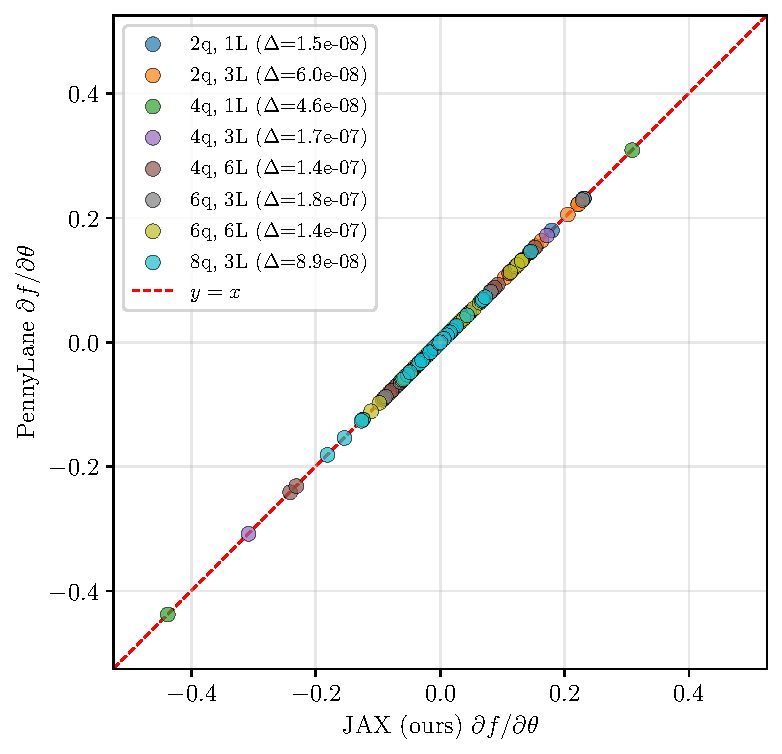
\includegraphics[width=0.7\textwidth]{figures/pqc_gradient_agreement.pdf}
\caption{Comparison of parameter gradients $\partial f / \partial \boldsymbol{\theta}_q$ computed by our JAX statevector implementation and PennyLane's \texttt{default.qubit} backend across eight circuit configurations (2--8 qubits, 1--6 layers). All values fall on the identity line $y = x$ with maximum absolute deviation $\Delta < 10^{-7}$, confirming numerical equivalence of the two implementations.}
\label{fig:S_pqc_gradient}
\end{figure}

\begin{figure}[H]
\centering
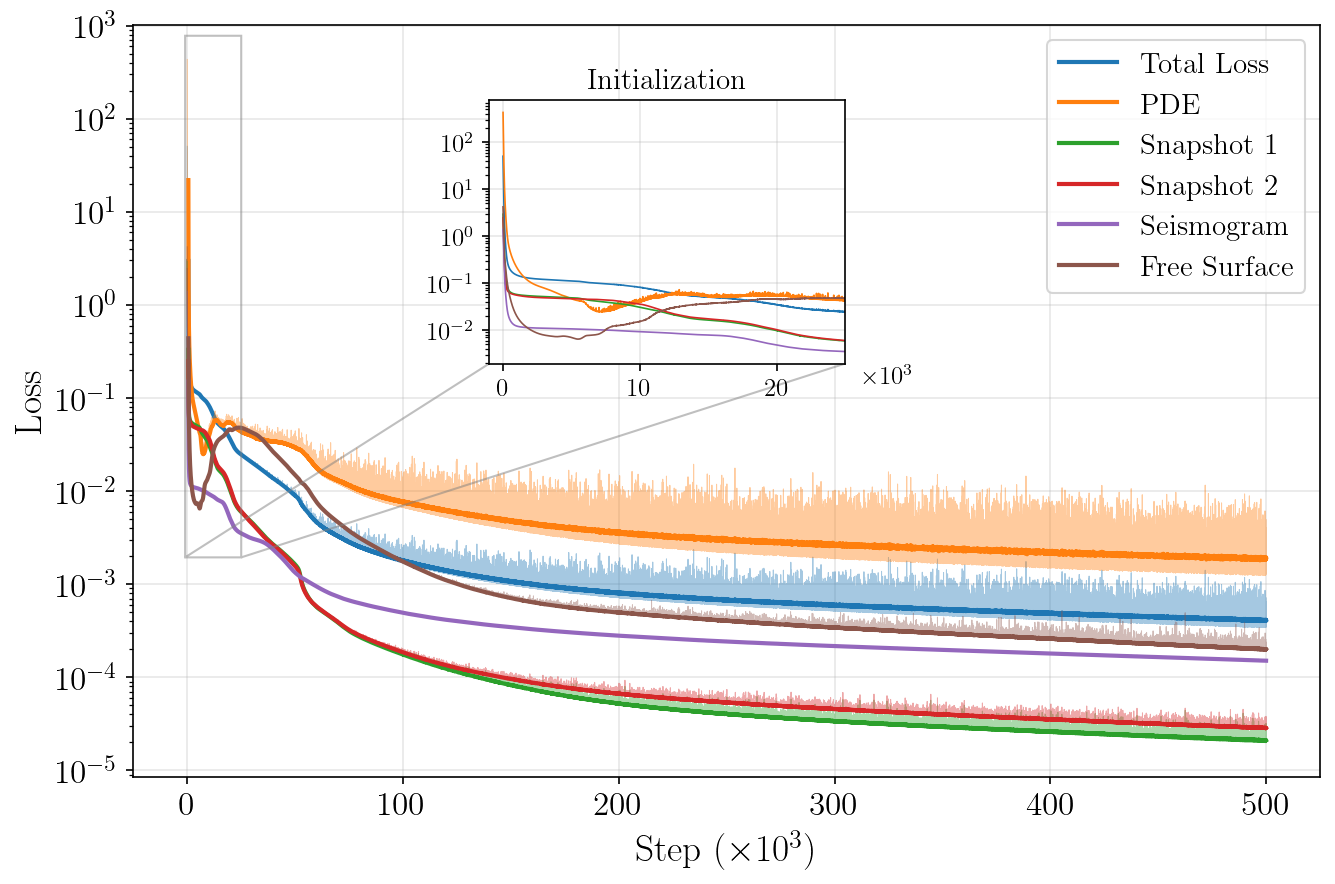
\includegraphics[width=0.8\linewidth]{../results/rasht/plots/metrics_losses.png}
\caption{Training loss decomposition for the classical FBPINN baseline on the anomaly benchmark: total loss, PDE residual, displacement-snapshot initial conditions (two components), seismogram misfit, and free-stress boundary condition, plotted versus training iteration. Inset: early-iteration behaviour showing rapid initial loss reduction.}
\label{fig:S_metrics_losses}
\end{figure}

\section*{Supplementary Tables}

\begin{table}[H]
\centering
\caption{Full hyperparameter variant sweep for the anomaly benchmark. $\mathcal{Q}(n_q^{\times n_L})$ denotes a parameterized quantum circuit with $n_q$ qubits and $n_L$ layers. Values marked ``--'' are identical to the \texttt{classical} baseline. Subdomains column shows $\phi(\cdot)$ for wavefield decomposition and $c(\cdot)$ for velocity decomposition.}
\label{tab:S_hyperparams_full}
\resizebox{\textwidth}{!}{%
\begin{tabular}{l l l c c c c c c c r}
\toprule
\textbf{Model} & \makecell{$\boldsymbol{\phi}$ \textbf{network}\\$(x,z,t)\!\to\!\phi$} & \makecell{$\boldsymbol{c}$ \textbf{network}\\$(x,z)\!\to\!c$} & \textbf{LR} & \textbf{Subs} & \textbf{Overlap} & $\boldsymbol{\lambda_\text{PDE}}$ & $\boldsymbol{\lambda_\text{IC}}$ & $\boldsymbol{\lambda_\text{seis}}$ & $\boldsymbol{\lambda_\text{BC}}$ & \textbf{\# Pars} \\\midrule
\texttt{classical} & $\mathcal{N}$: $32^{\times2}\!\to\!16^{\times2}$ & $\mathcal{N}$: $20^{\times5}$ & $10^{-4}$ & $\phi(5\!\times\!3\!\times\!5)$ & 0.35 & 0.1 & 1.0 & 1.0 & 0.1 & 151{,}836 \\
\midrule
\multicolumn{11}{l}{\emph{$\phi$-network size variants}} \\
\texttt{phi16x2} & $\mathcal{N}$: $16^{\times2}$ & -- & -- & -- & -- & -- & -- & -- & -- & 25{,}836 \\
\texttt{phi64x3} & $\mathcal{N}$: $64^{\times3}$ & -- & -- & -- & -- & -- & -- & -- & -- & 649{,}836 \\
\midrule
\multicolumn{11}{l}{\emph{$\phi$ subdomain decomposition variants}} \\
\texttt{sub3x2x3} & -- & -- & -- & $\phi(3\!\times\!2\!\times\!3)$ & -- & -- & -- & -- & -- & 37{,}779 \\
\texttt{sub8x4x8} & -- & -- & -- & $\phi(8\!\times\!4\!\times\!8)$ & -- & -- & -- & -- & -- & 514{,}017 \\
\midrule
\multicolumn{11}{l}{\emph{$c$-network size variants}} \\
\texttt{c10x2} & -- & $\mathcal{N}$: $10^{\times2}$ & -- & -- & -- & -- & -- & -- & -- & 150{,}226 \\
\texttt{c10x3} & -- & $\mathcal{N}$: $10^{\times3}$ & -- & -- & -- & -- & -- & -- & -- & 150{,}336 \\
\texttt{c20x3} & -- & $\mathcal{N}$: $20^{\times3}$ & -- & -- & -- & -- & -- & -- & -- & 150{,}996 \\
\texttt{c40x3} & -- & $\mathcal{N}$: $40^{\times3}$ & -- & -- & -- & -- & -- & -- & -- & 153{,}516 \\
\texttt{c40x5} & -- & $\mathcal{N}$: $40^{\times5}$ & -- & -- & -- & -- & -- & -- & -- & 156{,}796 \\
\texttt{c60x3} & -- & $\mathcal{N}$: $60^{\times3}$ & -- & -- & -- & -- & -- & -- & -- & 157{,}636 \\
\midrule
\multicolumn{11}{l}{\emph{Decomposed $c$-network variants}} \\
\texttt{c\_dec5x3} & -- & $\mathcal{N}$: $10^{\times2}$ & -- & \makecell{$\phi(5\!\times\!3\!\times\!5)$\\$c(5\!\times\!3)$} & -- & -- & -- & -- & -- & 152{,}340 \\
\texttt{c\_dec8x4} & -- & $\mathcal{N}$: $10^{\times2}$ & -- & \makecell{$\phi(5\!\times\!3\!\times\!5)$\\$c(8\!\times\!4)$} & -- & -- & -- & -- & -- & 154{,}907 \\
\texttt{c\_dec5x3\_20} & -- & $\mathcal{N}$: $20^{\times2}$ & -- & \makecell{$\phi(5\!\times\!3\!\times\!5)$\\$c(5\!\times\!3)$} & -- & -- & -- & -- & -- & 156{,}600 \\
\midrule
\multicolumn{11}{l}{\emph{Training hyperparameter variants}} \\
\texttt{lr5e4} & -- & -- & $5\!\times\!10^{-4}$ & -- & -- & -- & -- & -- & -- & -- \\
\texttt{lr5e5} & -- & -- & $5\!\times\!10^{-5}$ & -- & -- & -- & -- & -- & -- & -- \\
\texttt{overlap50} & -- & -- & -- & -- & 0.50 & -- & -- & -- & -- & -- \\
\texttt{wpde01\_wbc01} & -- & -- & -- & -- & -- & 0.01 & -- & -- & 0.01 & -- \\
\texttt{wpde1\_wbc1} & -- & -- & -- & -- & -- & 1.0 & -- & -- & 1.0 & -- \\
\midrule
\multicolumn{11}{l}{\emph{Quantum hybrid}} \\
\texttt{quantum} & $\mathcal{N}$: $32^{\times2}$ & $\mathcal{N}$: $20^{\times3}$ & -- & -- & -- & -- & -- & -- & -- & 101{,}812 \\
 & $\to$ $\mathcal{Q}$: $4^{\times2}$ & $\to$ $\mathcal{Q}$: $4^{\times2}$ & & & & & & & & \\
\bottomrule
\end{tabular}%
}
\end{table}


\end{document}
